\documentclass{assignment}
\ProjectInfos{在生活中感知材料的魅力}{GENS1004}{2020-2021学年第一学期}{第二次作业}{自然的鬼斧神工,科学的结构仿生}{陈稼霖}{45875852}
\begin{document}
\begin{ti}
    什么是仿生材料学?列举1种仿生材料及其应用。
\end{ti}
\begin{da}
    仿生材料学是指模仿生物的各种特点或特性而研制开发材料的学科,因为在自然选择下,生物的结构往往能进化出具有良好性能和功能的宏观和微观结构,因此仿照生物体结构制备的材料往往也能具有类似的优良属性。

    例如,人们从蜂窝中获得灵感,发明了仿生空心结构材料。蜂窝具有非常良好的结构性能:首先,蜂窝是以正六棱柱的单元紧密排列得到的,这种结构可以以非常少的材料占据非常大的体积,整体的密度很小,其次,蜂窝的结构可以很有效地传导引力,从而具有非常高的强度,最后,蜂窝的多孔结构具有巨大的表面积,从而有较好的吸附能力。

    根据蜂窝的特性,米其林公司设计了一款多孔轮胎(如图\ref{Michelim-porous-tire}),这款轮胎大部分的体积是中空,仅有少部分的骨架结构支撑,因此密度很轻,减少了车辆行驶的能耗,却具有非常高的强度。相比于充气轮胎,这款轮胎日常使用时不需要充气,除了使用过程中造成的磨损之外,不存在被戳破漏气的问题,因此具有较长的使用寿命。此外,在有积水的路面,轮胎的多孔结构可以使得遇到的积水很快地进入和排除轮胎,有效地防止了轮胎的打滑。

    蜂窝是一种牢固又轻巧的建筑,因此人们将类似的结构运用在建筑材料上,发明了蜂窝钢板(\ref{Honeycomb-steel-plate})、蜂窝状混凝土(如图\ref{Honeycomb-concrete})、蜂窝泡沫玻璃(如图\ref{Honeycomb-foam-glass})等建筑材料。以蜂窝状混凝土为例,蜂窝状混凝土密度小,常用蜂窝状混凝土的密度等级一般为$300-1200\mathrm{kg}/\mathrm{m}^3$,因此便于运输和安装,且减小了建筑自重。由于蜂窝状混凝土中含有大量封闭的细小孔隙,因此具有良好的保温隔热性能,可以为室内温控节约能源。蜂窝状混凝土还具有较好的隔音性。其中,混凝土是无机材料,不会燃烧,从而具有良好的耐火性,有利于建筑物防火。

    此外,蜂窝状的电极还可用于电池中,既有较好的吸附能力和通透性,便于离子的吸附和传输,还可减轻电池重量。
    \begin{figure}[H]
        \centering
        \subfigure[米其林多孔轮胎]{
            \label{Michelim-porous-tire}
            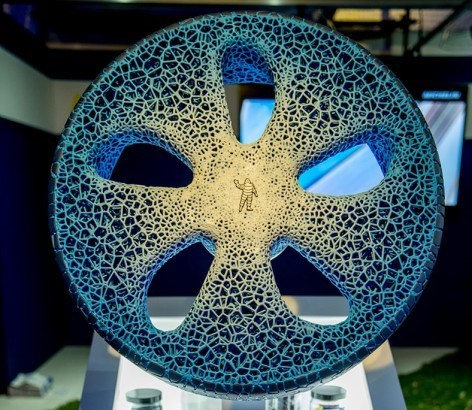
\includegraphics[width=.45\columnwidth]{Michelin-porous-tire.jpg}
        }
        \subfigure[蜂窝钢板]{
            \label{Honeycomb-steel-plate}
            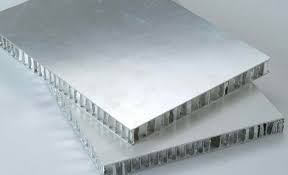
\includegraphics[width=.45\columnwidth]{Honeycomb-steel-plate.jpg}
        }
        \subfigure[蜂窝状混凝土]{
            \label{Honeycomb-concrete}
            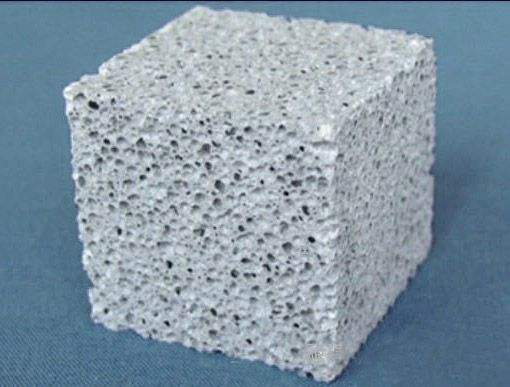
\includegraphics[width=.45\columnwidth]{Honeycomb-concrete.jpg}
        }
        \subfigure[蜂窝泡沫玻璃]{
            \label{Honeycomb-foam-glass}
            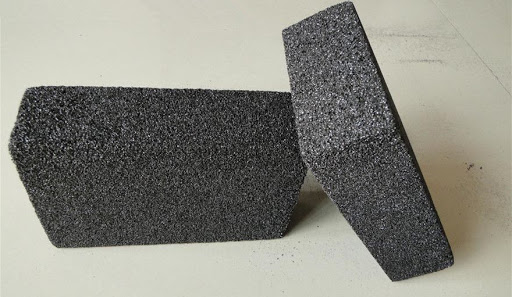
\includegraphics[width=.45\columnwidth]{Honeycomb-foam-glass.jpg}
        }
    \end{figure}

    又如,仿照莲花花瓣表面的纳米结构设计的纳米疏水衣物,可以有莲花一样“出淤泥而不染”的特性,可以大大减少衣物被污物附着的概率,使得衣物始终保持整洁而无需频繁洗换。
\end{da}

\begin{ti}
    贝壳是一种典型的有机-无机复合材料,具有特殊的结构并赋予其优良的力学性能,请进行具体描述。
\end{ti}
\begin{da}
    贝壳的基本结构大致可分为三部分,最外层为角质层,较薄,主要由硬质蛋白组成,中间为棱柱层,由柱状方解石排列组成,最内层为珍珠母层,是由$95\%$(体积比)的文石碳酸钙和$5\%$(体积比)的柔性生物高聚物(蛋白质和多糖)组成\cite{Zhao2017Preparation-and-application-of-shell-like-mother-of-pearl-layered-composite-material}\cite{Huang2008Research-on-Biomimetic-Composites-with-Shell-Nacre-Structure}\cite{Zhang2006Biomineralization-of-shell-nacre-and-its-enlightenment-to-biomimetic-materials}。

    贝壳珍珠母层的文石碳酸钙晶体片有序沉积所形成的多重微层结构是贝壳优良力学性能的关键来源。珍珠母层的文石碳酸钙晶体片是组成珍珠母层的基本结构单元,多为五、六边形,也存在菱形、混圆形和不规则多边形等多种形态,其宽度一般为$2\sim 20\,\mu$m,厚度约$0.3\sim 0.7\,\mu$m,文石碳酸钙晶体片横向生长使得临近的晶体片相互连接形成微层,微层间以厚约$30$ nm左右的有机基质连接构成珍珠母层\cite{Zhang2006Biomineralization-of-shell-nacre-and-its-enlightenment-to-biomimetic-materials}。这种用有机基质连接无机晶体片形成的微层结构又被称为“砖泥”结构。根据排列方式的不同,贝壳珍珠母层的转你结构可以分为薄板型结构(又称砖墙型结构)和圆柱型结构(堆垛型结构),前者主要存在与双壳类动物(如蛤、扇贝等)的贝壳中,后者主要存在于腹足类动物(如海螺等)的贝壳中\cite{Zhao2017Preparation-and-application-of-shell-like-mother-of-pearl-layered-composite-material}。介观层面上,在薄板型结构中,文石碳酸钙晶体片呈无规则堆叠,横向晶体片的连接处在不同层间相互交错(如图\ref{Shell}(b)(d));在圆柱型结构中,相邻层晶体片的沿垂直层的方向规则排列,其中心位置仅有$20\sim 30$ nm的微小偏移(如图\ref{Shell}(c)(e))\cite{Zhang2006Biomineralization-of-shell-nacre-and-its-enlightenment-to-biomimetic-materials}。微观层面上,文石碳酸钙晶体片表面是粗糙的,其上存在一些宽$10\sim 30$ nm,长$100\sim 200$ nm的凸起以及一些纳米尺度($<10$ nm)的小颗粒,这增强了层与层之间的摩擦作用,防止了层与层之间的滑移,且相邻两层文石碳酸钙晶体片之间被浸没在有机基质中的无机矿物质桥连接在一起,这同样防止了层与层之间的滑移与脱离\cite{Zhao2017Preparation-and-application-of-shell-like-mother-of-pearl-layered-composite-material}。

    \begin{figure}[H]
        \centering
        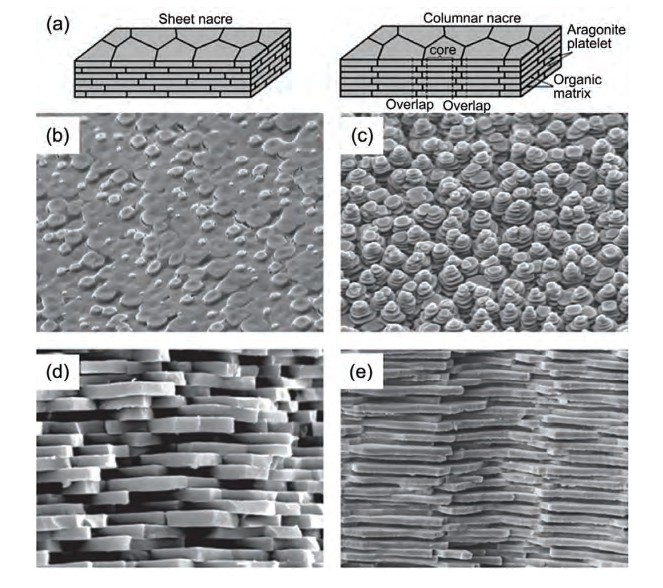
\includegraphics[width=.5\columnwidth]{Shell.jpg}
        \caption{贝壳珍珠母层“砖泥”结构的形貌。(a) 薄板型和圆柱型“砖泥”结构的示意图\cite{wang2012layered};(b)(d)薄板型结构的正面\cite{checa2009key}和截面\cite{barthelat2007mechanics}扫描隧道电子显微镜照片;(c)(e) 圆柱型结构的正面\cite{checa2009key}和截面\cite{rousseau2009dynamics}扫描电子显微镜照片。}
        \label{Shell}
    \end{figure}

    Meyers等人认为,当贝壳受到外界冲击时,无机片层的断裂和相邻无机片层之间的滑动(包括连接相邻无机片层的无机矿物质桥的断裂、无机片层粗糙表面引起的摩擦以及化学键的拉伸等)这两种机制都极大地耗散了外界冲击的能量\cite{meyers2008mechanical}(如图\ref{Shell-2}(c)-(e))。Espinosa等人利用原位原子力显微镜发现脆性的无机片层在纳米尺度会发生一定程度的弯曲,从而使材料的断裂面呈现起伏状,并且会随着片层的滑移而发生界面硬化,这也是一种耗散冲击能量的重要机制\cite{espinosa2011tablet}。此外,裂纹尖端塑性变形\cite{mayer2002rigid}\cite{rabiei2010failure}、裂纹偏转\cite{wang1995observations}\cite{wagner1992relationship}\cite{xia2015nanoasperity}、裂纹钝化\cite{menig2000quasi}、片层拔出\cite{meyers2013structural}(如图\ref{Shell-2}(b))、小尺寸结构单元\cite{gao2003materials}、无机片层表面的阶梯结构\cite{katti2005platelet}、有机基质的变形以及粘附作用\cite{menig2000quasi}和纳米结构的无机片层\cite{jackson1988mechanical}等都对能量的耗散有所贡献。这些能量耗散机制协同作用,造就了贝壳优良的力学性能。
    \begin{figure}[H]
        \centering
        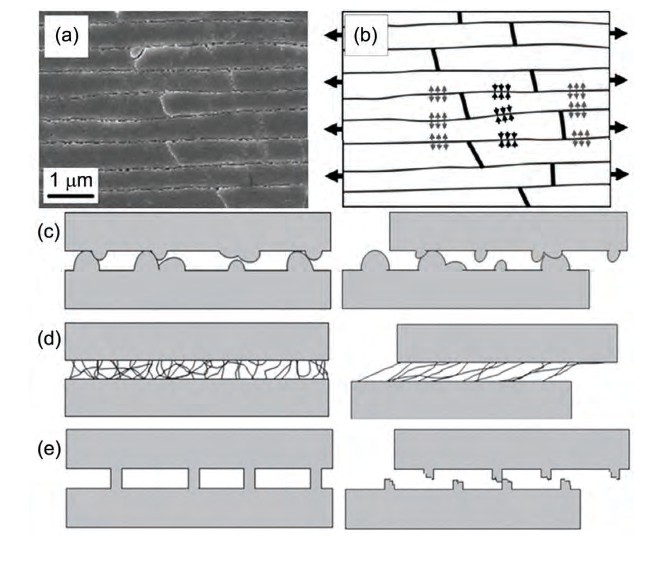
\includegraphics[width=.5\columnwidth]{Shell-2.jpg}
        \caption{贝壳珍珠母层的断裂机制。(a)(b) 微米尺度的断裂形貌和裂纹偏转示意图\cite{barthelat2007experimental};(c)-(e) 纳米尺度无机片层滑动示意图\cite{meyers2008mechanical}。}
        \label{Shell-2}
    \end{figure}
\end{da}

\begin{ti}
    鲨鱼皮有什么结构特征?仿生鲨鱼皮的泳衣是如何实现在水中减阻的?
\end{ti}
\begin{da}
    鲨鱼皮肤并不是一个光滑的表面,而是存在着大量的微小的齿状机构(如图\ref{Shark-skin}),这些微齿结构上含有大量疏水基团的蛋白基体,这些基体可以在鲨鱼皮肤表面形成一层较厚的疏水层。

    仿生鲨鱼皮的泳衣使用了仿鲨鱼皮减阻材料,它模仿了鲨鱼皮肤的齿状结构。首先,当水流流过仿鲨鱼皮减阻材料上面的每一个齿状结构,实际上就是流过每一个具有流线型的小结构。齿状的突起顺着水流的方向,具有导流的作用,能够尽量抑制湍流的产生。这样,在游动的过程中,水流能够尽量地贴着泳衣表面,而不会过早脱离而形成湍流,从而避免湍流带来的较大阻力。其次,仿鲨鱼皮材料上的疏水基团的蛋白基体使得材料表面形成一层疏水层,从而降低了水流对材料表面的粘滞阻力
    \begin{figure}[H]
        \centering
        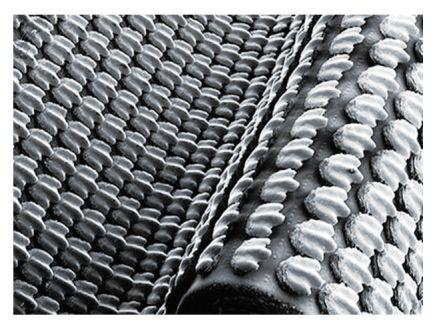
\includegraphics[width=.45\columnwidth]{Shark-skin.jpg}
        \caption{仿鲨鱼皮减阻材料}
        \label{Shark-skin}
    \end{figure}
\end{da}

\bibliographystyle{unsrt}
\bibliography{Assignment-2}
\end{document}